\documentclass[11pt]{article}
\usepackage[margin=1in]{geometry}
\usepackage[T1]{fontenc}
\usepackage{lmodern}
\usepackage{graphicx}
\usepackage{listings}
\usepackage{xcolor}
\usepackage{hyperref}
\usepackage{float}
\hypersetup{colorlinks=true, urlcolor=blue, linkcolor=black}

\lstset{
  basicstyle=\ttfamily\scriptsize,
  breaklines=true,
  columns=fullflexible,
  keepspaces=true,
  frame=single,
  framerule=0.3pt,
  rulecolor=\color{gray!60},
  backgroundcolor=\color{gray!5},
  showstringspaces=false,
}
\lstdefinestyle{py}{language=Python, basicstyle=\ttfamily\small}

\newcommand{\STUDENTNAME}{Anqi Li}
\newcommand{\GHUSER}{AnqiLi24}
\newcommand{\GHREPO}{https://github.com/AnqiLi24/elec576-assignment0}

\title{ELEC 576 / COMP 576 -- Assignment 0}
\author{\STUDENTNAME}
\date{\today}

\begin{document}
\maketitle

\section*{Task 1}
\lstinputlisting{task1_conda_info.txt}

\section*{Task 2}
\lstinputlisting{task2_transcript.txt}

\section*{Task 3}
\lstinputlisting{task3_transcript.txt}
\begin{figure}[H]
\centering
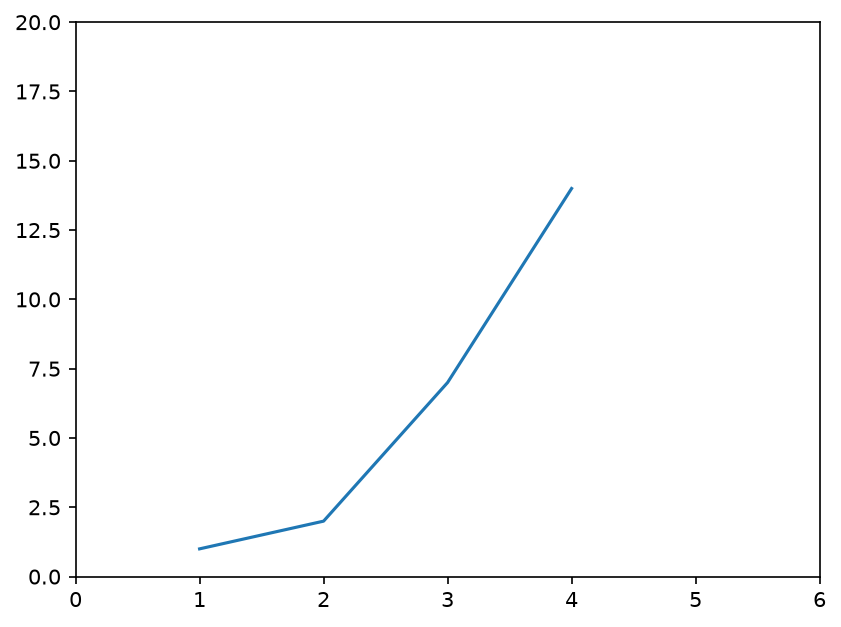
\includegraphics[width=0.65\linewidth]{task3_figure.png}
\end{figure}

\section*{Task 4}
\lstinputlisting[style=py]{../scripts/task4_plot.py}
\begin{figure}[H]
\centering
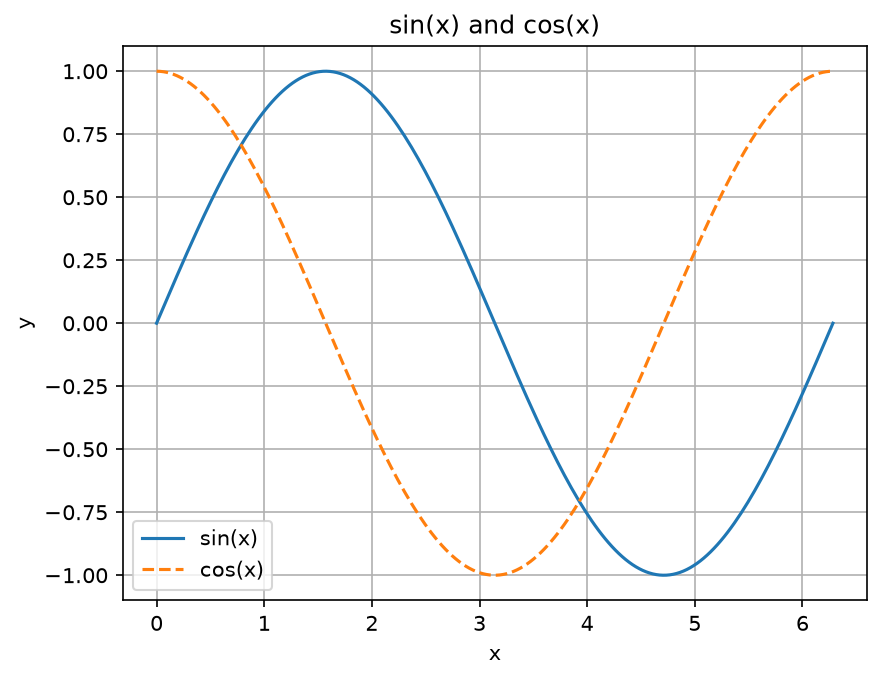
\includegraphics[width=0.7\linewidth]{task4_figure.png}
\end{figure}

\section*{Task 5}
GitHub account: \href{https://github.com/\GHUSER}{\GHUSER}

\section*{Task 6}
Project (VS Code), pushed to GitHub: \url{\GHREPO}

\end{document}
